\documentclass{beamer}

\title{The Impact of Anthropogenic Forcing on ENSO Amplitude}
\author{Ben Goldman}
\date{\today}

\usepackage{natbib}
\usepackage{tikz}
\usepackage{varwidth}
\usepackage{hyperref}
\usepackage[scale=1.4]{beamerposter}
\geometry{papersize={20in,48in}}
\usepackage{lipsum}

\usetikzlibrary{arrows,snakes,backgrounds}
\usetikzlibrary{positioning}
\tikzstyle{process}=[rectangle, draw=process, fill=process!20, line width = 0.3mm]
\tikzstyle{data}=[rectangle, draw=data, fill=data!20, line width = 0.3mm]
\tikzstyle{tight}=[node distance = 0.5in]
\tikzstyle{loose}=[node distance = 2in]
\definecolor{process}{HTML}{3d5f8f}
\definecolor{data}{HTML}{8f6d3d}

\usetheme{ben}

\newcommand{\myfig}[4]{
  \begin{figure}
    \centering
    \includegraphics[width=#3\textwidth]{figures/#1}
    \caption{#2}
    \label{fig:#4}
  \end{figure}
}
\renewcommand{\bibsection}{}

\begin{document}

\begin{frame}

  \begin{block}{Climate Change and Variability}
    \begin{figure}
      \begin{columns}
        \column{0.4\textwidth}
        \begin{itemize}
        \item Global warming
        \item Long-term trends vs short-term randomness
        \end{itemize}
        \caption{Global mean land air temperature in GISSTEMP 4 dataset. \citep{gistemp2019giss} and \citep{lenssen2019improvements}}
        \column{0.4\textwidth}
        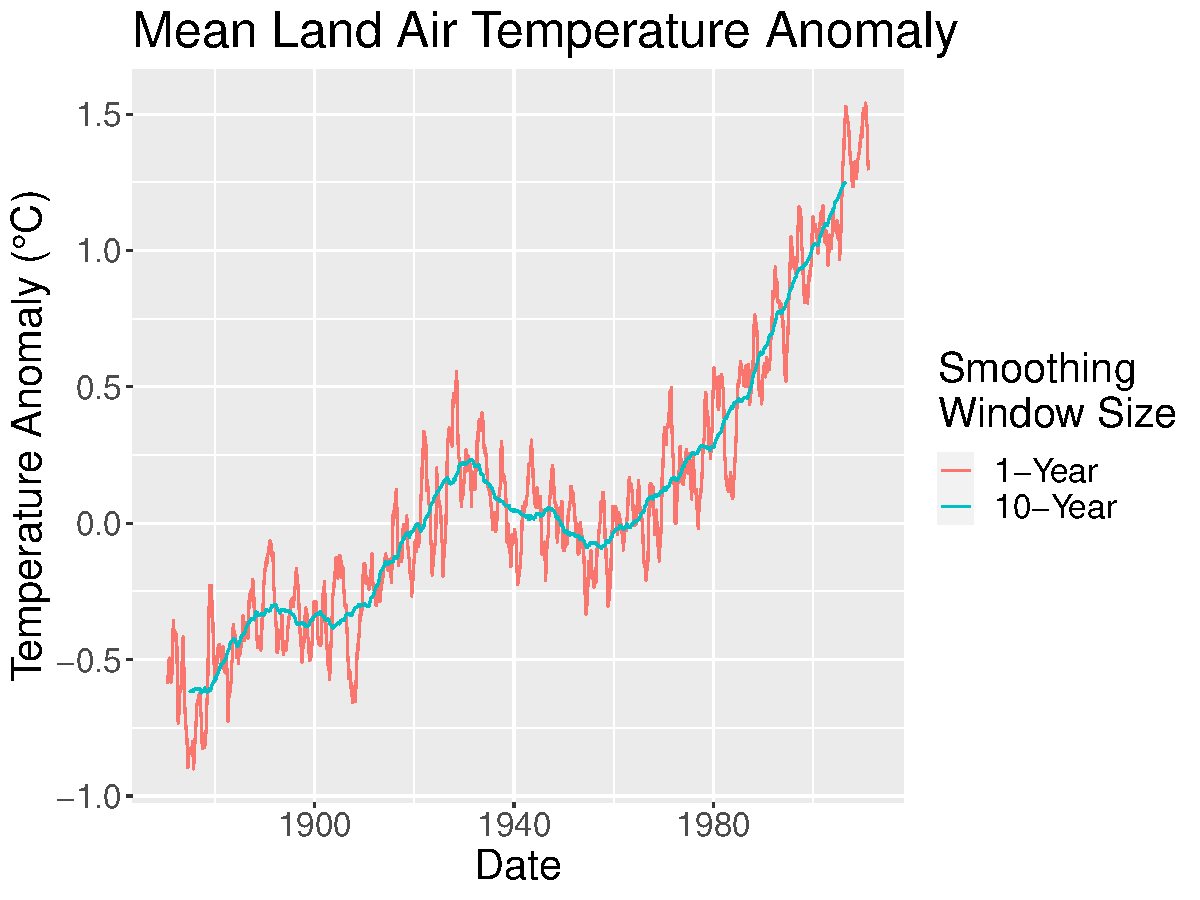
\includegraphics[width=1.0\textwidth]{figures/intro_fig_3.pdf}
      \end{columns}
    \end{figure}
  \end{block}
  \vfill

  \begin{block}{Climate Forcing}
    \begin{columns}
      \column{0.4\linewidth}
      \alert{Forcing}: any external factor that affects climate.
      \begin{description}
      \item[\alert{GHG}] Greenhouse gasses
      \item[\alert{AER}] Aerosols (natural: volcanic ash, artificial: smoke)
      \item[\alert{BMB}] Biomass burning
      \item[\alert{LULC}] Land use/cover (deforestation, desertification)
      \end{description}
      \column{0.4\linewidth}
      \myfig{greenhouse_Effect.jpg}{Factors that contribute to the greenhouse effect. \url{https://www.coolaustralia.org/the-greenhouse-effect-secondary}}{1.0}{this}
    \end{columns}
  \end{block}
  \vfill

  \begin{block}{El Niño (ENSO)}
    \begin{figure}
      \begin{columns}
        \column{0.4\textwidth}
        \begin{itemize}
        \item Warming and cooling of the Pacific Ocean.
        \item Affects human societies through temperature and rainfall. \citep{ropelewski1987global}
        \item May be affected by climate change.
        \end{itemize}
        \caption{Comparison of SST anomaly between 1975 La Niña event and 1997 El Niño event in HadISST 1 dataset. \citep{rayner2003global}}
        \column{0.4\textwidth}
        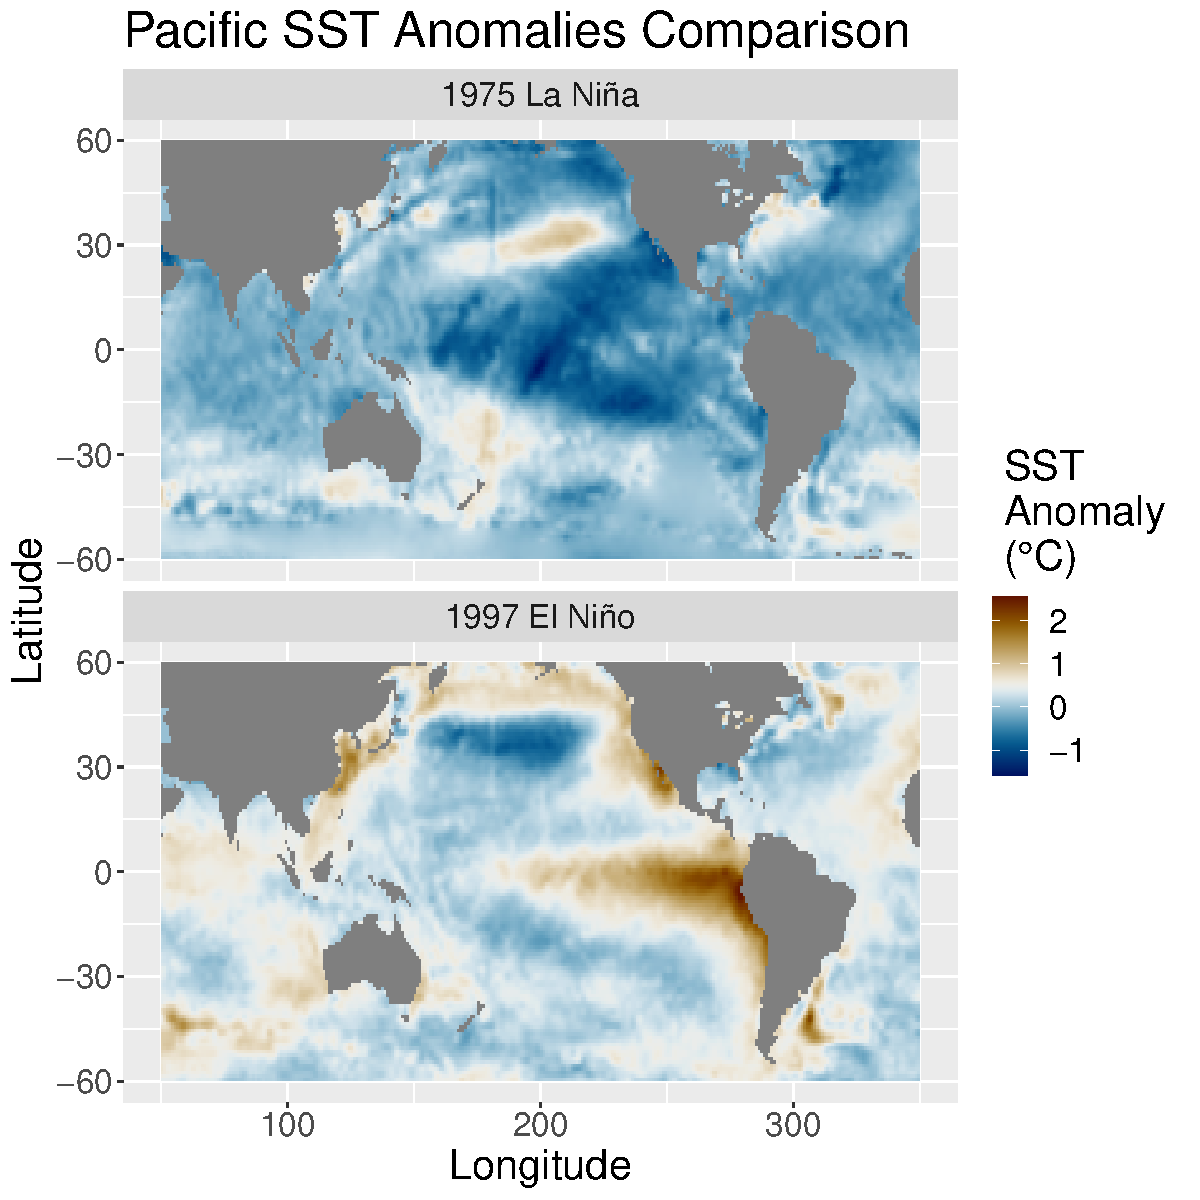
\includegraphics[width=1.0\textwidth]{figures/intro_fig.pdf}
      \end{columns}
    \end{figure}
  \end{block}
  \vfill

  \begin{block}{Review of Literature}
    \begin{itemize}
    \item ENSO's properties observed vary across different decades. \citep{lubbecke2014assessing}.
    \item ENSO responds to external forcing.
    \item Weakened ENSO during the Ice Age due to reduced CO$_2$ levels \citep{zhu2017reduced}.
    \item Models show possible increasing ENSO activity in the future \citep{zheng2017response} and \citep{maher2018enso}.
    \end{itemize}
  \end{block}
  \vfill

  \begin{block}{Gap and Questions}
    \begin{itemize}
    \item Little research using a large ensemble to examine the effect of individual factors on ENSO.
    \item Considerable disagreement between studies on whether ENSO will strengthen or weaken due to global warming
    \end{itemize}
    \begin{description}
    \item[What?] Do the CESM1 and CESM2 predict increased or decreased ENSO intensity in the future?
    \item[Why?] Is the predicted increase (or decrease) due to human activities?
    \item[How?] What processes are causing greenhouse gasses and aerosols to affect ENSO?
    \end{description}
  \end{block}
  \vfill

  \begin{block}{Model Setup (Data)}
    \begin{itemize}
    \item CESM1 \citep{kay2015community} and CESM2 \citep{danabasoglu2020community}
    \item Predicts climate over 21st century with global warming.
    \item 40-50 simulations per ensemble.
    \item Control simulation with pre-1850 forcing levels.
    \item Single forcing ensembles that represent influence of single factor.
    \end{itemize}
  \end{block}
  \vfill

  \begin{block}{Measuring ENSO Intensity}
    \begin{center}
      \begin{tikzpicture}[node distance = 2.0in and 0.2\linewidth, line width = 1.5mm]
        \node [data] (input) {
          \begin{varwidth}{4.0in}
            External forcing
          \end{varwidth}};
        \node [process] (model) [right=of input] {
          \begin{varwidth}{4.0in}
            CESM1\\and\\CESM2
          \end{varwidth}};
        \node [data] (output) [right=of model] {
          \begin{varwidth}{4.0in}
            Sea surface temperature (SST)
          \end{varwidth}};
        \node [data] (nino) [below=of input] {
          \begin{varwidth}{4.0in}
            Niño 4.0 index
          \end{varwidth}};
        \node [process] (variance) [right=of nino] {
          \begin{varwidth}{4.0in}
            Windowed\\variance
          \end{varwidth}};
        \node [data] (intensity) [right=of variance] {
          \begin{varwidth}{4.0in}
            ENSO intensity
          \end{varwidth}};
        \draw [->] (input) to (model);
        \draw [->] (model) to (output);
        \draw [->] (output) to [out = 210, in = 30] (nino);
        \draw [->] (nino) to (variance);
        \draw [->] (variance) to (intensity);
      \end{tikzpicture}
    \end{center}
  \end{block}

\end{frame}

\begin{frame}{References}
  \bibliographystyle{apalike}
  \bibliography{references.bib}
\end{frame}

\end{document}
